\documentclass[12pt]{article}
\usepackage[utf8]{inputenc}
%\usepackage[margin=1in]{geometry}
\usepackage{parskip}
\usepackage{fullpage}
\usepackage{tabularx}
\usepackage{float}
\usepackage{graphicx}
\title{Lab III\\\normalsize{PLSC 501}}
\author{Oner Yigit}
\date{\today}

\begin{document}

\maketitle

\section{Part I—Model Specification}
\subsection{Predicted Values and Residuals}
\begin{figure}[H]
\centering
\includegraphics[width=0.99\textwidth]{figure123.pdf}
\end{figure}

\subsection{Evaluation and Heteroskedasticity}

Figure 1 shows that true values of \textit{Murder Rate} and predicted values are similar. They together linearly increase. This is a good thing because we want our predicted values, $\hat{y}$, to be as similar as true values.

Figure 2 shows that there is significant difference between residuals, $y- \hat{y}$. For instance, some predicted values of \textit{murder rate} between $6-8$ seems very different from our true values, meaning that we predict different murder rate, and the distance between $y$ and $\hat{y}$ is as high as $6$. The same logic also apply to Figure 3, where we look at unemployment rate and residuals. While unemployment rate around 7 for an observation, the residuals is around 6, meaning that we are 6 point away from the unemployment rate. 

\textit{Heteroskedasticity}. I perform Bresuch-Pagan test. 

Null Hypothesis: The model is Homoscedastic. 

Alternative Hypothesis: The model is not Homoscedastic.

Bresuch-Pagan test gives $<05$. Therefore, we reject the null Hypothesis, which means that our model \textit{does} have heteroskedasticity issue.


It seems that the model predict yhat very well based on the Figure 1. However,  I not sure if the model is good enough given the residuals are spread around.  
\vspace{1cm}

\section{Part II—Out of Sample Plots}

\vspace{0.5cm}

\subsection{Hypotheses (Hypothetical)}


\textbf{H1:} One Unit increase in polity score is more likely to increase the number of protests. \\

\textbf{H2:} One Unit increase in population is more likely to increase the number of protests.\\

\textbf{H3:} One unit increase in GDP is more likely to decrease the number of protests.\\

\textbf{H4:} An increase in the number of employed people is more likely to decrease the number of protests\\

\textbf{H5:} One unit increase in Household Consumption is more likely to decrease the number of protests.\\

\textbf{H6: } Compare to other regions, the number of protests will be low.

\subsection{Regression Model}


\begin{table}[H] \centering
\caption{Effects on Number of Protests}
\begin{tabular}{@{\extracolsep{5pt}}lc}
\\[-1.8ex]\hline
\hline \\[-1.8ex]
& \multicolumn{1}{c}{\textit{DV: Number of Protests}} \
\cr \cline{1-2}
\\[-1.8ex] & \multicolumn{1}{c}{Model I} \\\\[-1.8ex] & (1) \\
\hline \\[-1.8ex]
 Polity Score & 0.082$^{***}$ \\
  & (0.015) \\
 Population (Million) & 0.010$^{***}$ \\
  & (0.003) \\
 GDP & 0.000$^{***}$ \\
  & (0.000) \\
 \# of Employed & -0.027$^{***}$ \\
  & (0.007) \\
 Household Consumption & -1.123$^{***}$ \\
  & (0.354) \\
 Europe (dummy) & 0.294$^{}$ \\
  & (0.228) \\
 Constant & 3.105$^{***}$ \\
  & (0.181) \\
\hline \\[-1.8ex]
 Observations & 3,523 \\
 $R^2$ & 0.071 \\
 Adjusted $R^2$ & 0.070 \\
 Residual Std. Error & 5.136(df = 3516)  \\
 F Statistic & 44.996$^{***}$ (df = 6.0; 3516.0) \\
\hline
\hline \\[-1.8ex]
\textit{Note:} & \multicolumn{1}{r}{$^{*}$p$<$0.1; $^{**}$p$<$0.05; $^{***}$p$<$0.01} \\
\end{tabular}
\end{table}

\subsection{Effect of Polity Score}
\begin{figure}[H]
  \centering
  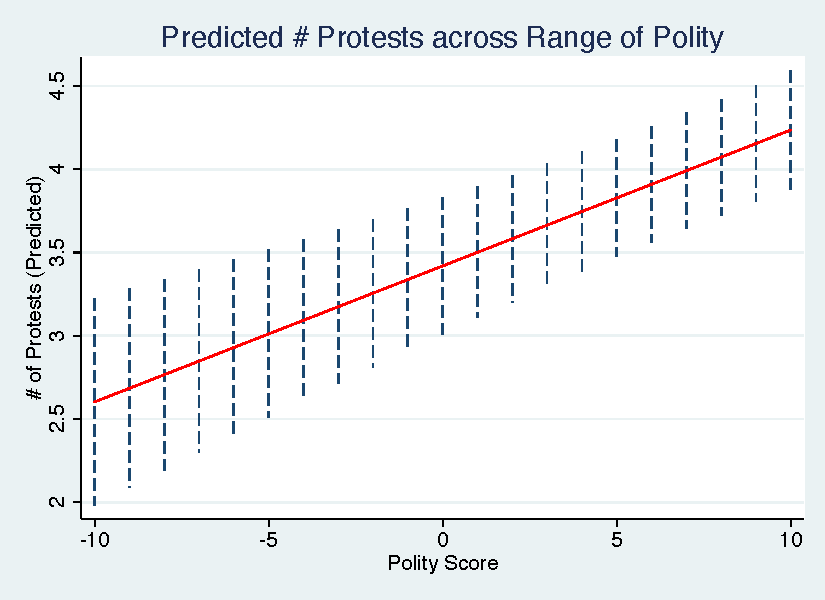
\includegraphics[width=0.99\textwidth]{polity1.pdf}
  \end{figure}
  
This graph shows the relationship or the effect of polity score on predicted number of protests when we hold other variables in the model at their mean. We can see that the more polity score increases so does our predicted number of protests. Therefore, polity score has a positive effect on number of protests, and it is statistically significant.  


\subsection{Effect of Polity Score comparing low and high Household Consumption}
\begin{figure}[H]
  \centering
  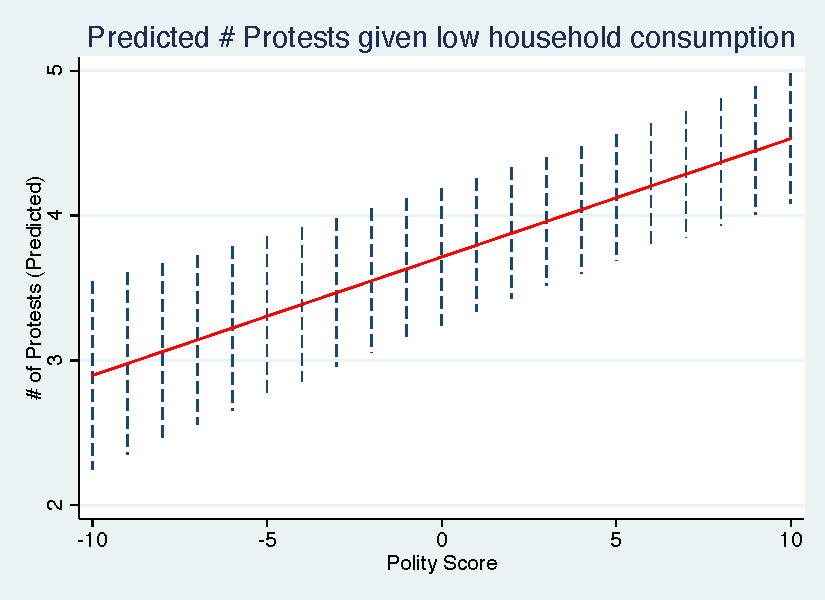
\includegraphics[width=0.75\textwidth]{polity10.pdf}
  \end{figure}

  \begin{figure}[H]
    \centering
    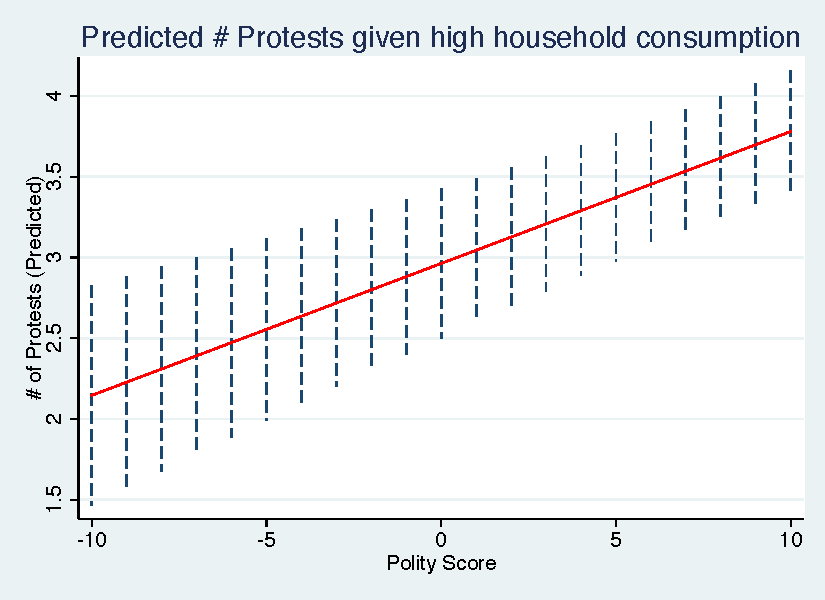
\includegraphics[width=0.75\textwidth]{polity90.pdf}
    \end{figure}

    
The plots show that high household consumption has a significantly higher effect on protests than low household consumption, but the effect of each level of consumption group gets more positive as regime type becomes more democratic. Our goal is to show the effect of polity score for multiple groups of household consumption levels.  

\end{document}
